\documentclass{standalone}
\usepackage{tikz}
\usetikzlibrary{patterns, positioning}

\begin{document}
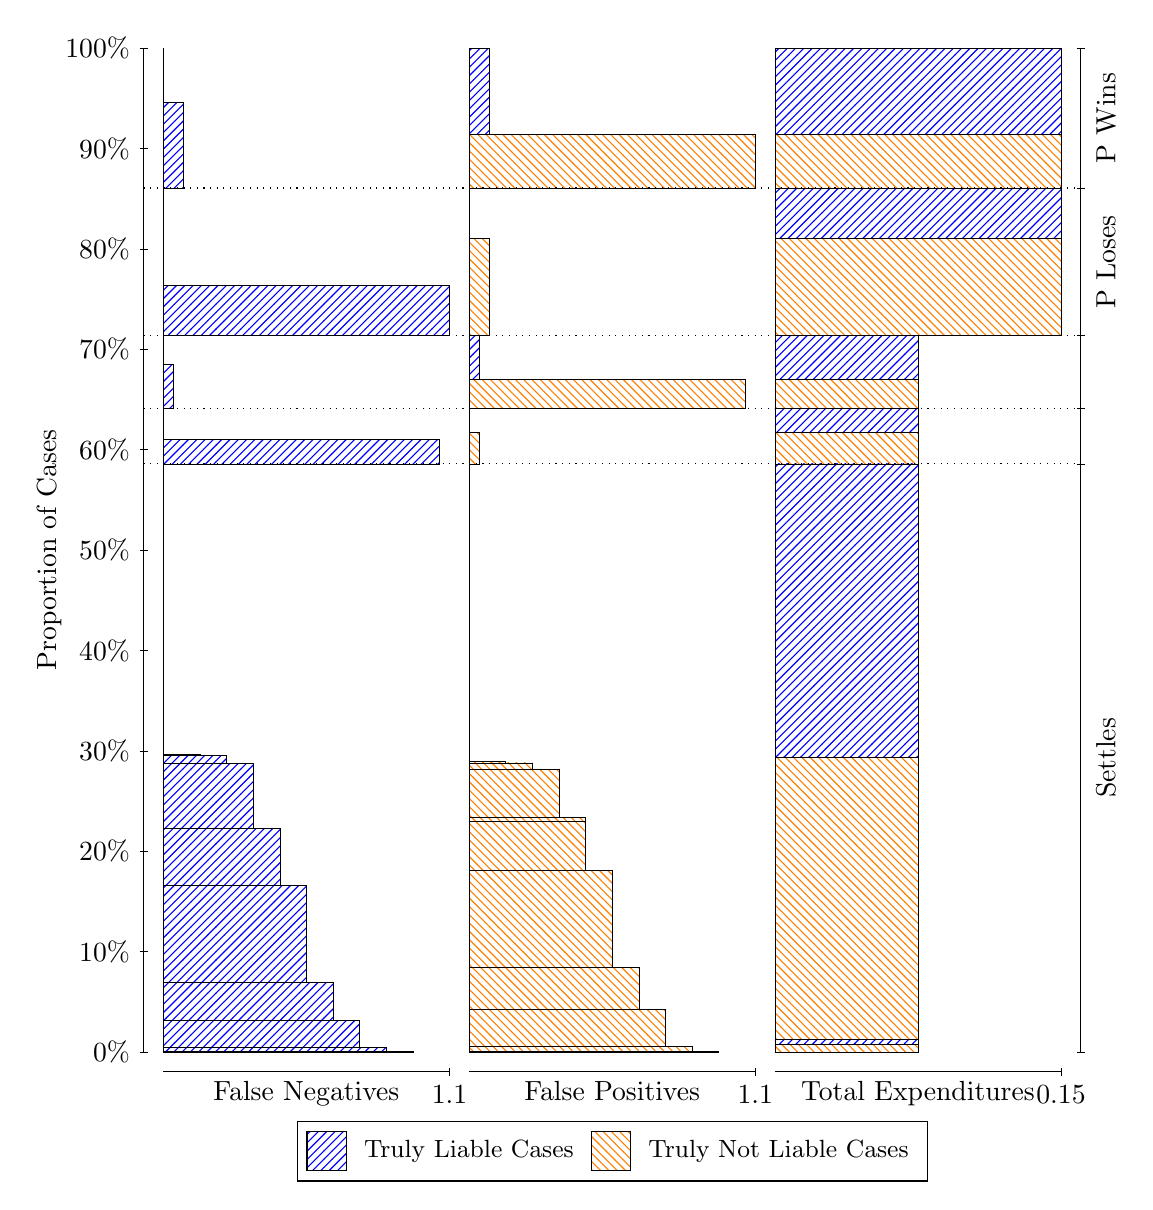
\begin{tikzpicture}
\draw[black, very thin] (1.5,1.75) -- (1.5,14.5);
\node[rotate=90, anchor=center] at (0.3, 8.125) {Proportion of Cases};
\draw[black, very thin] (1.45,1.75) -- (1.55,1.75);
\node[anchor=east] at (1.45, 1.75) {0\%};
\draw[black, very thin] (1.45,3.025) -- (1.55,3.025);
\node[anchor=east] at (1.45, 3.025) {10\%};
\draw[black, very thin] (1.45,4.3) -- (1.55,4.3);
\node[anchor=east] at (1.45, 4.3) {20\%};
\draw[black, very thin] (1.45,5.575) -- (1.55,5.575);
\node[anchor=east] at (1.45, 5.575) {30\%};
\draw[black, very thin] (1.45,6.85) -- (1.55,6.85);
\node[anchor=east] at (1.45, 6.85) {40\%};
\draw[black, very thin] (1.45,8.125) -- (1.55,8.125);
\node[anchor=east] at (1.45, 8.125) {50\%};
\draw[black, very thin] (1.45,9.4) -- (1.55,9.4);
\node[anchor=east] at (1.45, 9.4) {60\%};
\draw[black, very thin] (1.45,10.675) -- (1.55,10.675);
\node[anchor=east] at (1.45, 10.675) {70\%};
\draw[black, very thin] (1.45,11.95) -- (1.55,11.95);
\node[anchor=east] at (1.45, 11.95) {80\%};
\draw[black, very thin] (1.45,13.225) -- (1.55,13.225);
\node[anchor=east] at (1.45, 13.225) {90\%};
\draw[black, very thin] (1.45,14.5) -- (1.55,14.5);
\node[anchor=east] at (1.45, 14.5) {100\%};

\draw[black, very thin] (13.4,1.75) -- (13.4,14.5);
\draw[black, very thin] (13.35,1.75) -- (13.45,1.75);
\node[anchor=west] at (13.35, 1.75) {};
\draw[black, very thin] (13.35,9.2189) -- (13.45,9.2189);
\node[anchor=west] at (13.35, 9.2189) {};
\draw[black, very thin] (13.35,9.9254) -- (13.45,9.9254);
\node[anchor=west] at (13.35, 9.9254) {};
\draw[black, very thin] (13.35,10.847) -- (13.45,10.847);
\node[anchor=west] at (13.35, 10.847) {};
\draw[black, very thin] (13.35,12.722) -- (13.45,12.722);
\node[anchor=west] at (13.35, 12.722) {};
\draw[black, very thin] (13.35,14.5) -- (13.45,14.5);
\node[anchor=west] at (13.35, 14.5) {};

\draw[black, very thin, pattern color=blue, pattern=north east lines] (1.75,1.75) rectangle (4.9186,1.7621);
\draw[black, very thin, pattern color=blue, pattern=north east lines] (1.75,1.7621) rectangle (4.5806,1.8107);
\draw[black, very thin, pattern color=blue, pattern=north east lines] (1.75,1.8107) rectangle (4.2426,2.1493);
\draw[black, very thin, pattern color=blue, pattern=north east lines] (1.75,2.1493) rectangle (3.9047,2.6375);
\draw[black, very thin, pattern color=blue, pattern=north east lines] (1.75,2.6375) rectangle (3.5667,3.8669);
\draw[black, very thin, pattern color=blue, pattern=north east lines] (1.75,3.8669) rectangle (3.2287,4.5898);
\draw[black, very thin, pattern color=blue, pattern=north east lines] (1.75,4.5898) rectangle (2.8907,5.4119);
\draw[black, very thin, pattern color=blue, pattern=north east lines] (1.75,5.4119) rectangle (2.5527,5.5204);
\draw[black, very thin, pattern color=blue, pattern=north east lines] (1.75,5.5204) rectangle (2.2147,5.5314);
\draw[black, very thin, pattern color=orange, pattern=north west lines] (1.75,5.5314) rectangle (1.75,9.2189);
\draw[black, very thin, pattern color=blue, pattern=north east lines] (1.75,9.2189) rectangle (5.2566,9.5267);
\draw[black, very thin, pattern color=orange, pattern=north west lines] (1.75,9.5267) rectangle (1.75,9.9254);
\draw[black, very thin, pattern color=blue, pattern=north east lines] (1.75,9.9254) rectangle (1.8767,10.479);
\draw[black, very thin, pattern color=orange, pattern=north west lines] (1.75,10.479) rectangle (1.75,10.847);
\draw[black, very thin, pattern color=blue, pattern=north east lines] (1.75,10.847) rectangle (5.3833,11.487);
\draw[black, very thin, pattern color=orange, pattern=north west lines] (1.75,11.487) rectangle (1.75,12.722);
\draw[black, very thin, pattern color=blue, pattern=north east lines] (1.75,12.722) rectangle (2.0035,13.814);
\draw[black, very thin, pattern color=orange, pattern=north west lines] (1.75,13.814) rectangle (1.75,14.5);
\draw[black, very thin, pattern color=orange, pattern=north west lines] (5.6333,1.75) rectangle (8.8019,1.7591);
\draw[black, very thin, pattern color=orange, pattern=north west lines] (5.6333,1.7591) rectangle (8.464,1.8238);
\draw[black, very thin, pattern color=orange, pattern=north west lines] (5.6333,1.8238) rectangle (8.126,2.2941);
\draw[black, very thin, pattern color=orange, pattern=north west lines] (5.6333,2.2941) rectangle (7.788,2.8245);
\draw[black, very thin, pattern color=orange, pattern=north west lines] (5.6333,2.8245) rectangle (7.45,4.0568);
\draw[black, very thin, pattern color=orange, pattern=north west lines] (5.6333,4.0568) rectangle (7.112,4.6742);
\draw[black, very thin, pattern color=orange, pattern=north west lines] (5.6333,4.6742) rectangle (7.112,4.7252);
\draw[black, very thin, pattern color=orange, pattern=north west lines] (5.6333,4.7252) rectangle (6.774,5.3389);
\draw[black, very thin, pattern color=orange, pattern=north west lines] (5.6333,5.3389) rectangle (6.436,5.4206);
\draw[black, very thin, pattern color=orange, pattern=north west lines] (5.6333,5.4206) rectangle (6.0981,5.4375);
\draw[black, very thin, pattern color=blue, pattern=north east lines] (5.6333,5.4375) rectangle (5.6333,9.2189);
\draw[black, very thin, pattern color=orange, pattern=north west lines] (5.6333,9.2189) rectangle (5.7601,9.6176);
\draw[black, very thin, pattern color=blue, pattern=north east lines] (5.6333,9.6176) rectangle (5.6333,9.9254);
\draw[black, very thin, pattern color=orange, pattern=north west lines] (5.6333,9.9254) rectangle (9.1399,10.293);
\draw[black, very thin, pattern color=blue, pattern=north east lines] (5.6333,10.293) rectangle (5.7601,10.847);
\draw[black, very thin, pattern color=orange, pattern=north west lines] (5.6333,10.847) rectangle (5.8868,12.083);
\draw[black, very thin, pattern color=blue, pattern=north east lines] (5.6333,12.083) rectangle (5.6333,12.722);
\draw[black, very thin, pattern color=orange, pattern=north west lines] (5.6333,12.722) rectangle (9.2667,13.408);
\draw[black, very thin, pattern color=blue, pattern=north east lines] (5.6333,13.408) rectangle (5.8868,14.5);
\draw[black, very thin, pattern color=orange, pattern=north west lines] (9.5167,1.75) rectangle (11.333,1.8486);
\draw[black, very thin, pattern color=blue, pattern=north east lines] (9.5167,1.8486) rectangle (11.333,1.9094);
\draw[black, very thin, pattern color=orange, pattern=north west lines] (9.5167,1.9094) rectangle (11.333,5.4982);
\draw[black, very thin, pattern color=blue, pattern=north east lines] (9.5167,5.4982) rectangle (11.333,9.2189);
\draw[black, very thin, pattern color=orange, pattern=north west lines] (9.5167,9.2189) rectangle (11.333,9.6176);
\draw[black, very thin, pattern color=blue, pattern=north east lines] (9.5167,9.6176) rectangle (11.333,9.9254);
\draw[black, very thin, pattern color=orange, pattern=north west lines] (9.5167,9.9254) rectangle (11.333,10.293);
\draw[black, very thin, pattern color=blue, pattern=north east lines] (9.5167,10.293) rectangle (11.333,10.847);
\draw[black, very thin, pattern color=orange, pattern=north west lines] (9.5167,10.847) rectangle (13.15,12.083);
\draw[black, very thin, pattern color=blue, pattern=north east lines] (9.5167,12.083) rectangle (13.15,12.722);
\draw[black, very thin, pattern color=orange, pattern=north west lines] (9.5167,12.722) rectangle (13.15,13.408);
\draw[black, very thin, pattern color=blue, pattern=north east lines] (9.5167,13.408) rectangle (13.15,14.5);
\draw[black, dotted] (1.5,9.2189) -- (13.4,9.2189);
\draw[black, dotted] (1.5,9.9254) -- (13.4,9.9254);
\draw[black, dotted] (1.5,10.847) -- (13.4,10.847);
\draw[black, dotted] (1.5,12.722) -- (13.4,12.722);
\draw[black, very thin] (1.75,1.5) -- (5.3833,1.5);
\node[anchor=north] at (3.5667, 1.5) {False Negatives};
\draw[black, very thin] (5.3833,1.45) -- (5.3833,1.55);
\node[anchor=north] at (5.3833, 1.45) {1.1};

\draw[black, very thin] (5.6333,1.5) -- (9.2667,1.5);
\node[anchor=north] at (7.45, 1.5) {False Positives};
\draw[black, very thin] (9.2667,1.45) -- (9.2667,1.55);
\node[anchor=north] at (9.2667, 1.45) {1.1};

\draw[black, very thin] (9.5167,1.5) -- (13.15,1.5);
\node[anchor=north] at (11.333, 1.5) {Total Expenditures};
\draw[black, very thin] (13.15,1.45) -- (13.15,1.55);
\node[anchor=north] at (13.15, 1.45) {0.15};

\node[black, centered, rotate=90] at (13.72, 5.4845) {Settles};


\node[black, centered, rotate=90] at (13.72, 11.785) {P Loses};
\node[black, centered, rotate=90] at (13.72, 13.611) {P Wins};

\draw (7.449999999999999,1.5) node[draw=none] (baseCoordinate) {};
\begin{scope}[align=center]
        \matrix[scale=0.5, draw=black, below=0.5cm of baseCoordinate, nodes={draw}, column sep=0.1cm]{
            \node[rectangle, draw, minimum width=0.5cm, minimum height=0.5cm, pattern=north east lines, pattern color=blue] {}; &
            \node[draw=none, font=\small] (B) {Truly Liable Cases}; &
            \node[rectangle, draw, minimum width=0.5cm, minimum height=0.5cm, pattern=north west lines, pattern color=orange] {}; &
            \node[draw=none, font=\small] (B) {Truly Not Liable Cases}; \\
            };
\end{scope}

\end{tikzpicture}
\end{document}